\chapter{Background}

In this chapter I am going to introduce the reader to the concepts that are necessary to understand the research presented in this thesis. The chapter is divided into three sections. The first section provides an overview of Variational Autoencoders (VAEs) and their applications. The second section introduces Vector Quantized VAEs (VQ-VAEs). The third section introduces the concept of Multitask learning. 

\section{VAEs}

Variational Autoencoders (VAEs), first introduced in 2013 by Kingma and Welling\cite{kingma2013autoencoding}, have become a prominent class of generative models in the field of machine learning.  At their core, VAEs consist of an encoder network with parameters $\phi$ that maps data points $x$ into a latent space $z$ and a decoder network with parameters $\theta$ that generates data $\hat{x}$ from latent representations\cite{Kingma_2019}. 

The key innovation that makes VAEs work is the introduction of a probabilistic interpretation of the latent space. More specifically, VAEs assume that the latent space $z$ is a random variable that follows a certain prior distribution $p(z)$, which is typically a Gaussian distribution and that the mapping from the latent space to the data space is also probabilistic\cite{kingma2013autoencoding}.

The optimization target for VAEs is the evidence lower bound (ELBO) which is: \[ L_{\theta, \phi}(x) = \mathbb{E}_{q_{\phi}(z|x)} [\log p_{\theta}(x, z) - \log q_{\phi}(z|x)] \] where $q_{\phi}(z|x)$ is the encoder distribution, $p_{\theta}(z, x)$ is the decoder distribution and $p(z)$ is the prior distribution. 

The ELBO can be also written as a sum of two terms: \[ L_{\theta, \phi}(x) = - D_{KL}(q_{\phi}(z|x) || p(z)) + \mathbb{E}_{q_{\phi}(z|x)} [\log p_{\theta}(x|z)] \]
And if we look at the Monte Carlo estimate of the ELBO, we can see that the first term is the regularization term and the second term is the reconstruction term:
\[ L_{\theta, \phi}(x) = - D_{KL}(q_{\phi}(z|x) || p(z)) + \frac{1}{L} \sum_{l=1}^{L} \log p_{\theta}(x|z^{(l)}) \]
where $z^{(l)} \sim q_{\phi}(z|x)$. The regularization term is the Kullback-Leibler divergence between the encoder distribution and the prior distribution. The regularization term encourages the encoder distribution to be close to the prior distribution. The reconstruction term is the reconstruction error of the decoder. The reconstruction term encourages the decoder to reconstruct the input data as accurately as possible.

The individual datapoint ELBO and it's gradient in general is intractable to compute. However, unbiased estimates of the ELBO and its gradients can be obtained using the reparametrization trick, which is described in the next section\cite{Kingma_2019}.


\subsection{Reparametrization Trick}

The Reparametrization trick also  is a crucial component of VAEs. It is used to make the ELBO differentiable w.r.t the parameters of the encoder $\phi$ and decoder $\theta$. The notion is based on the fact we can define a random variable $z \sim q_{\phi}(z|x)$ as a deterministic, differentiable function of a random variable $\epsilon$ and the parameters $\phi$ such that $z = g_{\phi}(\epsilon, x)$, where the distribution of $\epsilon$ is independent of $\phi$ and $x$: $\epsilon \sim p(\epsilon)$. With this parameterization, the expectation w.r.t $q_{\phi}(z|x)$ can be rewritten as an expectation w.r.t. $p(\epsilon)$: \[ L_{\theta, \phi}(x) = \mathbb{E}_{q_{\phi}(z|x)} [\log p_{\theta}(x, z) - \log q_{\phi}(z|x)] \]
\[ = \mathbb{E}_{p(\epsilon)} [\log p_{\theta}(x, g_{\phi}(\epsilon, x)) - \log q_{\phi}(g_{\phi}(\epsilon, x)|x)] \] which is differentiable w.r.t $\phi$ and $\theta$.



\subsection{Gaussian VAEs}

Altough Gaussian VAEs are just a special case of VAEs, they are the most common type of VAEs. Gaussian VAEs assume that the prior distribution $p(z)$ is a centered Gaussian distribution $ p(z) = \mathcal{N}(0, I)$. They also assume that the decoder distribution $p_{\theta}(x|z)$ is a Gaussian distribution whose distribution parameters are computed from z with a single fully connected layer: 
\[ p_{\theta}(x|z) = \mathcal{N}(f_{\theta}(z), \sigma_{\theta}(z)) \]
where $f_{\theta}(z)$ is the mean and $\sigma_{\theta}(z)$ is the standard deviation of the Gaussian distribution. Whilst there is a lot of freedom in the form $q_{\phi}(z|x)$ can take, Gaussian VAEs assume that $q_{\phi}(z|x)$ is also a Gaussian distribution with an approximately diagonal covariance matrix: 
\[ q_{\phi}(z|x) = \mathcal{N}(\mu_{\phi}(x), \sigma_{\phi}(x)) \]
where $\mu_{\phi}(x)$ and $\sigma_{\phi}(x)$ are the mean and standard deviation of the Gaussian distribution which are computed by the encoder network.

To sample $z$ from $q_{\phi}(z|x)$, we can use the reparametrization trick described in the previous section: \[ z = \mu_{\phi}(x) + \sigma_{\phi}(x) \odot \epsilon \] where $\epsilon \sim \mathcal{N}(0, I)$ is a random variable sampled from a standard Gaussian distribution.

When applying these assumptions to the ELBO, we get the following expression: \[ L_{\theta, \phi}(x) = - D_{KL}(q_{\phi}(z|x) || p(z)) + \frac{1}{L} \sum_{l=1}^{L} \log p_{\theta}(x|z^{(l)}) \]
\[ = - D_{KL}(\mathcal{N}(\mu_{\phi}(x), \sigma_{\phi}(x)) || \mathcal{N}(0, I)) + \frac{1}{L} \sum_{l=1}^{L} \log \mathcal{N}(x|f_{\theta}(z^{(l)}), \sigma_{\theta}(z^{(l)})) \]
where $f_{\theta}(z^{(l)}) = f_{\theta}(\mu_{\phi}(x) + \sigma_{\phi}(x) \odot \epsilon^{(l)})$ and $\sigma_{\theta}(z^{(l)}) = \sigma_{\theta}(\mu_{\phi}(x) + \sigma_{\phi}(x) \odot \epsilon^{(l)})$ and $\epsilon^{(l)} \sim \mathcal{N}(0, I)$.

However, the loss function to be minimized for VAE's usually used in practise is quite different from the ELBO negative. The function that is used in practice consists of: Mean Squared Error (MSE) reconstruction loss, KL divergence regularization loss and a constant $\beta$ that controls the importance of the regularization term:
\[ L = \frac{1}{n} \sum_{i=1}^{n} ||x_i - f_{\theta}(z^{(i)}) ||^2 + D_{KL}(\mathcal{N}(\mu_{\phi}(x), \sigma_{\phi}(x)) || \mathcal{N}(0, I)) \]
where $f_{\theta}(z^{(i)}) = f_{\theta}(\mu_{\phi}(x_i) + \sigma_{\phi}(x_i) \odot \epsilon^{(i)})$ and $\epsilon^{(i)} \sim \mathcal{N}(0, I)$. The MSE reconstruction loss is used because maximizing the Gaussian likelihood is approximately equivalent to minimizing the MSE reconstruction loss:

\begin{equation} \label{eqMSE}
    \begin{split}
        p(x|z) &= \mathcal{N}(x|f(z), \sigma(z)) \\
        \log p(x|z) &\sim  \log \mathcal{N}(x|f(z), \sigma(z)) \\
        \log p(x|z) &\sim  \log \frac{1}{\sqrt{2 \pi \sigma(z)^2}} \exp(-\frac{(x - f(z))^2}{2 \sigma(z)^2}) \\
        \log p(x|z) &\sim  \log \exp(-\frac{(x - f(z))^2}{2 \sigma(z)^2}) \\
        \log p(x|z) &\sim  - \frac{1}{2 \sigma(z)^2} * (x - f(z))^2 \\
        \log p(x|z) &\sim  -  (x - f(z))^2 \\
    \end{split}
\end{equation}

In the figure belowe \ref{VAEFigure} there is a visualization of the architecture of Gaussian VAEs.


\begin{figure}[H]
    \centering
    \makebox[\textwidth]{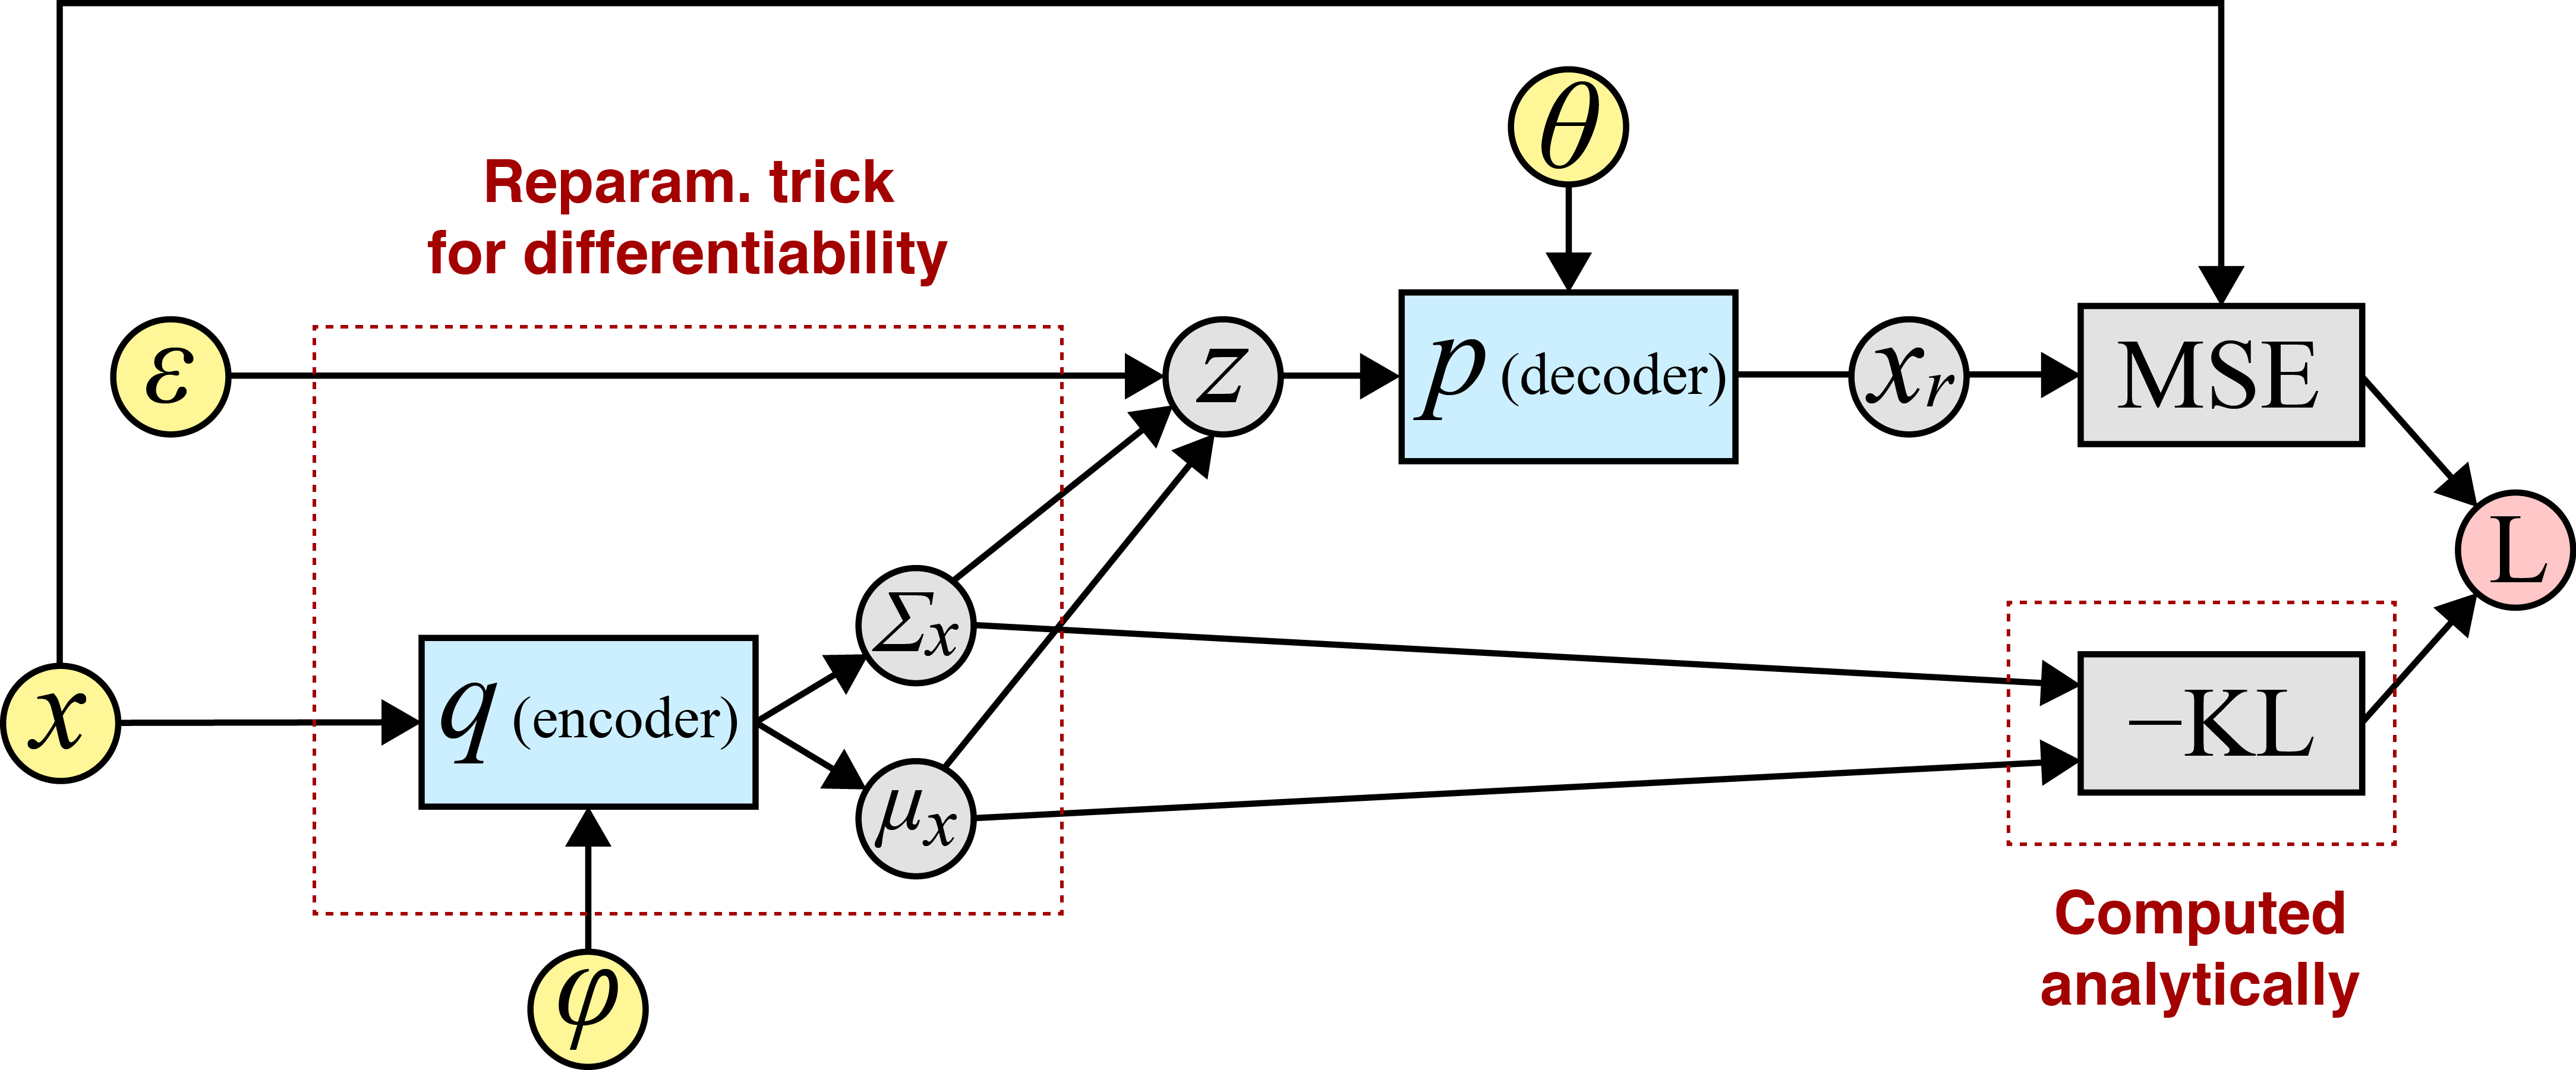
\includegraphics[width=\textwidth]{figures/vae}}

    \caption{ The architecture of VAEs.}
  	\medskip 
	\hspace*{15pt}\hbox{\scriptsize Credit: Aäron van den Oord et al.}
    \label{VAEFigure}
\end{figure}

\pagebreak

\section{Vector Quantized VAEs}

Vector Quantized VAEs (VQ-VAEs) are a variant of VAEs that were introduced in 2017 by Aäron van den Oord et al\cite{vqvae}. VQ-VAEs use discrete latent variables with a new way of training, which was inspired by vector quantization (VQ). Both posterior and prior distributions are categorical, and the samples are drawn from these distributions index an embedding table\cite{vqvae}. These embeddings are then used to reconstruct the input data. The architecture of VQ-VAEs is shown in figure \ref{VQVAEFigure}.

\subsection {Discrete Latent Variables}

VQ-VAEs define a latent embedding space $ e \in \mathbb{R}^{K \times D} $, where $K$ is the number of embeddings and $D$ is the dimension of each latent embedding vector. The model takes an input $x$, which is passed through the encoder producing output $z_e(x)$, as shown in figure \ref{VQVAEFigure}. 
The discrete latent variables $z$ are then calculated by nearest neighbour lookup in the embedding space: \[ z = \argmin_{k} || z_e(x) - e_k ||^2 \] where $e_k$ is the $k$-th embedding vector in the embedding space. The decoder then takes the discrete latent variables $z$ and produces the output $\hat{x}$.

\begin{figure}[H]
    \centering
    \makebox[\textwidth]{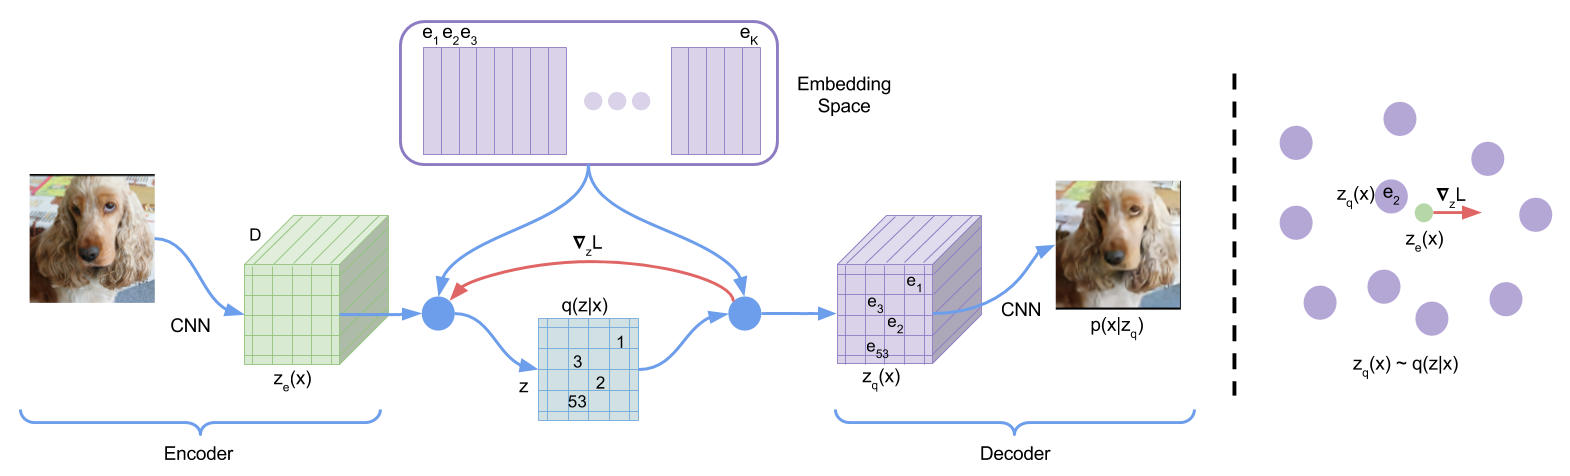
\includegraphics[width=\textwidth]{figures/vq_vae}}

    \caption{On the left side there is a figure describing the VQ-VAE architecture. On the right side there is visualization of the latent space whilst training. The figure is taken from \cite{vqvae}.}
  	\medskip 
	\hspace*{15pt}\hbox{\scriptsize Credit: Aäron van den Oord et al.}
    \label{VQVAEFigure}
\end{figure}


